An \emph{ordinary differential equation} is an equation which governs the evolution of a function $u : I \to V$ mapping an interval $I \subseteq \R$ to a finite-dimensional vector space $V$ known as the \emph{state space}. Abstractly, they are equations which take the form 
	\begin{equation}
		G(u, \partial_t u, \dots, \partial_t^k u, t) = 0.
		\tag{nLin}
		\label{eq:nLin}
	\end{equation}	
for some given function $G : V^{k + 1} \times I \to W$, where $W$ is another finite-dimensional vector space. We are interested in the \emph{initial data problem}, also known as the Cauchy problem, in which we aim to find a $k$-times continuously differentiable solution satisfying \emph{initial data conditions},
	\begin{align*}
		u_{|t = 0}
			&= u_0, \\
		\partial_t u_{|t = 0}
			&= u_1,\\
			&\vdots \\
		\partial_t^{k - 1} u_{|t = 0}	
			&= u_{k - 1}	
	\end{align*}
for some $u_0, u_1, \dots, u_{k - 1} \in V$. 	

\subsection{Types of equations}

The most general form of an ODE is a fully \emph{non-linear} equation (\ref{eq:nLin}). This is a \emph{system of equations} when the codomain of $G$ has more than one dimension, otherwise it is a \emph{scalar equation}. If the number of equations $\dim W$ exceeds the degrees of freedom $\dim V$, then the equation is \emph{over-determined}, in which case one may require additional constraints on any initial data before a solution can be found. Conversely if there are fewer equations than degrees of freedom, the equation is \emph{under-determined}, and so there may be a multiplicity of solutions for any given data. 

We will only consider ODE which are \emph{fully determined}: the number of equations coincides with the degrees of freedom. In this case, assuming some non-degeneracy conditions, any non-linear ODE can be reduced to a \emph{quasi-linear} ODE, that is, one which is linear with respect to the highest-order derivatives. 

\begin{proposition}[Reduction to quasi-linear]
	Let $G : V^{k + 1} \times I \to V$ is continuously differentiable, and suppose that $u_k \mapsto G(u_0, u_1, \dots, u_{k - 1}, u_k, 0)$ is invertible. Then there exists there exists $F: V^{k + 1} \times I \to V$ such that
		\begin{equation}
			 \partial_t^{k + 1} u = F(u, \partial_t u, \dots, \partial_t^{k} u, t).\tag{qLin}\label{eq:qLin}
		\end{equation}	
\end{proposition}

\begin{proof}
	We differentiate the equation (\ref{eq:nLin}), obtaining by the chain rule
		\[ \partial_t G + \sum_{j = 0}^{k - 1} D_{u_j} G \cdot \partial_t^{j + 1} u + D_{u_k} G \cdot \partial_t^{k + 1} u = 0.\]
	Rearranging and inverting the matrix $D_{u_k} G$ gives the result. 	
\end{proof}


When the function $G$ in (\ref{eq:nLin}) does not depend on the time-variable $t$, we say the ODE is \emph{autonomous}, otherwise we say it is \emph{non-autonomous}. Autonomous ODEs enjoy the property of \textit{time-translation-invariance}, i.e. if $t \mapsto u(t)$ is a solution, then so is $t \mapsto u(t - t_0)$. Every non-autonomous system can be converted into an autonomous one by embedding the time-variable into the state-space. 

\begin{proposition}[Reduction to autonomy]
	Every non-autonomous ODE,
		\begin{align}
			G(u, \partial_t u, \dots, \partial_t^k u, t) 
			&= 0,\tag{nAut}\label{eq:nAut}
		\end{align}	
	can be reduced to an autonomous ODE,
		\begin{align}
			\widetilde G(\widetilde u, \partial_t \widetilde u, \dots, \partial_t^k \widetilde u)
			&= 0. \tag{Aut}\label{eq:Aut}
		\end{align}	
\end{proposition}

\begin{proof}
	Define $\widetilde u : I \to V \times I$ and $\widetilde G : (V \times I)^{k + 1} \times I \to W \times I$ by 
		\begin{align*}
			\widetilde u (t)
				&:= (u(t), t),\\
			\widetilde G((u_0, s_0), (u_1, s_1), \dots, (u_k, s_k))
				&:= (G(u_0, \dots, u_k), s_1 - 1).
		\end{align*}
	A routine check shows that every solution to (\ref{eq:nAut}) is a solution to (\ref{eq:Aut}), and conversely, every solution to (\ref{eq:Aut}) is a solution to (\ref{eq:nAut}) modulo time-translation. 
\end{proof}



\begin{example}
	The quasilinear non-autonomous ODE
		\[ \partial_t u = F(t, u) \]
	is equivalent to the \textit{system} of autonomous ODE
		\begin{align*}
			\partial_t u(t) 
				&= F(s, t), \\
			\partial_t s(t)
				&= 1. 	
		\end{align*}
\end{example}

The \emph{order} of an ODE refers to the order of the highest derivative occurring in the equation. Any $k$-th order system can be reduced to a first-order system at the cost of multiplying the degrees of freedom by $k$. 

\begin{proposition}[Reduction of order]
	Every $k$-th order quasi-linear ODE, 
		\begin{align}
			\partial_t^k  u
				&= F(u, \partial_t u, \dots \partial^{k - 1} u),
				\tag{$k^{\text{th}}$}
				\label{eq:kth}
		\end{align}
	can be reduced to a first-order quasi-linear ODE,
		\begin{align}
			\partial_t \widetilde u
				&= \widetilde F (u). 
				\tag{$1^{\text{st}}$}
				\label{eq:1st}
		\end{align}
\end{proposition}

\begin{proof}
	Set $\widetilde u : I \to V^k$ and $\widetilde F: V^k \to V^k$ to be
		\begin{align*}
			\widetilde u 
				&:= (u, \partial_t u, \dots, \partial_t^{k - 1} u) ,\\
			\widetilde F (u_0, \dots, u_{k - 1})
				&= (u_1, \dots, u_{k - 1}, F(u_0, \dots, u_{k - 1}))	.
		\end{align*}	
	Then $\widetilde u$ is a continuously differentiable solution to the first-order equation (\ref{eq:1st}) if and only if $u$ is $k$-times continuously differentiable solution to the $k$-th order equation (\ref{eq:kth}). 	
\end{proof}


\subsection{Notions of a solution}

With these reductions at hand, we focus our attention to the study of the initial data problem for first-order quasi-linear systems of equations on $\R^n$, 
\begin{equation}
	\begin{split}
		\partial_t u 	&= F(u), \\
		u_{|t = 0}		&= u_0.
	\end{split}\tag{IDP}	\label{eq:idp}
\end{equation}
If we assume the non-linearity is analytic, then one could hope to solve the ODE by differentiating the equation to obtain a recurrence relation for $\partial_t^k u$, and then show the corresponding formal power series for $u$ converges. Indeed, this is the approach of the Cauchy-Kowalevskaya theorem. However, without such strong assumptions on $F$, it is not clear how one could solve (\ref{eq:idp}) by ``classical'' (read: undergraduate calculus) methods. 

To get around this, often times it becomes easier to solve an equation by ``weakening'' the notion of a solution, giving access to tools from functional analysis when dealing with PDEs, or metric space topology in the case of ODEs. We say that a solution $u : [0, T] \to \R^n$ to (\ref{eq:idp}) is a
\begin{itemize}
	\item a \emph{classical solution} if $u \in C^1_\loc ([0, T])$ and satisfies the initial data problem for all $t \in [0, T]$ using the classical notion of the derivative. 
	
	\begin{figure}[h]
		\begin{center}
			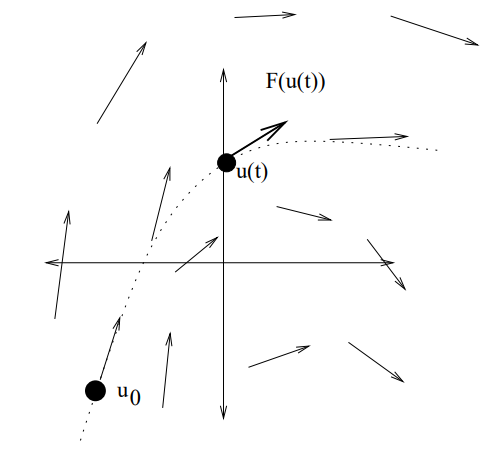
\includegraphics[scale = 0.5]{classical}
			\caption{The non-linearity $F(u)$ is regarded as a \textit{force} which governs the velocity $\partial_t u$ and thereby the evolution of the solution $u$.}
		\end{center}
	\end{figure}
	
	\item a \emph{strong solution} if $u \in C^0_\loc ([0, T])$ and solves the initial data problem in the integral sense that 
					\[ u(t) = u_0 + \int_0^t F(u(s))\, ds \]
				for all $t \in [0, T]$. 	
				
	\begin{figure}[h]
		\begin{center}
			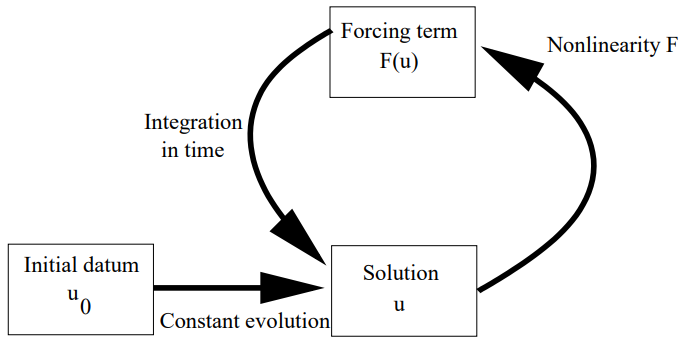
\includegraphics[scale = 0.5]{strong}
			\caption{The relationship between the solution $u$ and the non-linearity $F(u)$ can be viewed as a \textit{feedback loop} in which the solution influences the non-linearity, and vice versa.}
		\end{center}
	\end{figure}	
	
	\item a \emph{weak solution} if $u \in L^\infty ([0, T])$ which solves the initial data problem in the sense of distributions, i.e.
				\[ \int_0^T u(t) \psi (t) \, dt = u_0 \int_0^T \psi (t) \, dt + \int_0^T \psi (t) \left(\int_0^T F(u(s)) \, ds\right) dt \]
			for all test functions $\psi \in C_c^\infty ([0, T])$. 	
\end{itemize}

\begin{proposition}[Equivalence of notions]
	Let $F: \R^n \to \R^n$ be continuous and $u_0 \in \R^n$, then the notions of classical, strong, and weak solutions to the initial data problem (\ref{eq:idp}) are equivalent. 
\end{proposition}

\begin{proof}
	 It is clear that a classical solution is strong by the fundamental theorem of calculus, and that a strong solution is weak. If $u$ is a weak solution, we know that $t \mapsto F(u(t))$ is bounded and measurable and therefore
	\[ t \mapsto \int_0^t F(u(s)) \, ds \]
is Lipschitz continuous. Choose $\psi$ to be approximations to the identity concentrated at $t$, the weak formulation implies that
	\[ u(t) = u_0 + \int_0^t F(u(s)) \, ds \]
for a.e. $t$. It follow that $u$ is Lipschitz up to modification on a measure zero set, so it is a strong solution. Then $t \mapsto F(u(t))$ is in fact continuous, and so by the fundamental theorem of calculus $u \in C^1_\loc ([0, T])$ and solves the initial data problem classically. 
\end{proof}


\subsection{Well-posedness}

One should think of the initial data problem as governing the time evolution $\partial_t u$ of a physical state $u$ starting from an initial condition $u_0$. Not all ODEs are of physical relevance, though if it were to have one, and indeed these are the equations we care about, then we expect it to have the following properties:
	\begin{itemize}
		\item Existence: if a physical phenomenon is governed by an ODE, then it should correspond to a solution. 
		
		\item Uniqueness: physical reality is deterministic, the past determines the future, so there should only be one solution for each initial data. 
		
		\item Continuous dependence on initial data: the evolution of a physical phenomenon is stable under perturbations, so the solution should depend continuously on the initial data. 
	\end{itemize}
If the initial data problem (\ref{eq:idp}) satisfies these three criterion, then we say it is \emph{well-posed}. The concept of well-posedness was introduced by Hadamard in \cite{hadamard} as an attempt to clarify the link between differential equation and physics. 

For a more precise statement, we need to specify the space in which we look for solutions to the initial data problem, the time interval of existence, and the topology on the space of solutions. We say well-posedness is
	\begin{itemize}
		\item \emph{conditional} vs. \emph{unconditional} if well-posedness holds only in a subset $X \subseteq C^0 ([0, T] \to \R^n)$ vs. the entire space $X = C^0 ([0, T] \to \R^n)$, 
		
		\item \emph{local} vs \emph{global} if well-posedness holds only for finite time $[0, T]$ vs. infinite time $[0, \infty)$, 
		
		\item $C^{k, \alpha}$ if the solution map $u_0 \mapsto u$ is $C^{k, \alpha}$-differentiable, where differentiability is taken in a Frechet sense. 
	\end{itemize}
Our starting point will be to show local conditional $C^0$-well-posedness, which states that	for any $u_0^* \in \Omega$, there exists a time $T > 0$ and an open ball $B \subseteq \Omega$ containing $u_0^*$ and a subset $X \subseteq C^0([0, T] \to \R^n)$ such that for each $u_0 \in B$ there exists a unique strong solution $u \in X$, and furthermore the solution map $u_0 \mapsto u$ is continuous. 
